\subsection{IU2 Agendar Citas del paciente}

\subsubsection{Objetivo}
Permitir al paciente agendar una cita en la fecha, hora y consultorio que desee, siempre y cuando haya disponibilidad.

\subsubsection{Diseño}
Esta pantalla aparece al presionar la opción ``Agendar cita'' en el menu lateral del paciente

\begin{figure}[htbp!]
    \centering
        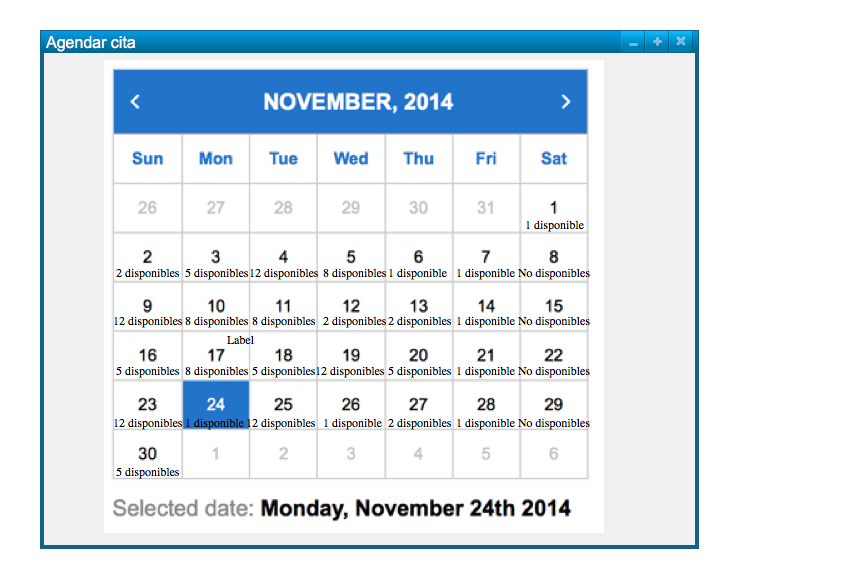
\includegraphics[width=0.8\textwidth]{images/UI2A}
    \caption{Pantalla UI2A Agendar cita}
\end{figure}

\begin{figure}[htbp!]
    \centering
        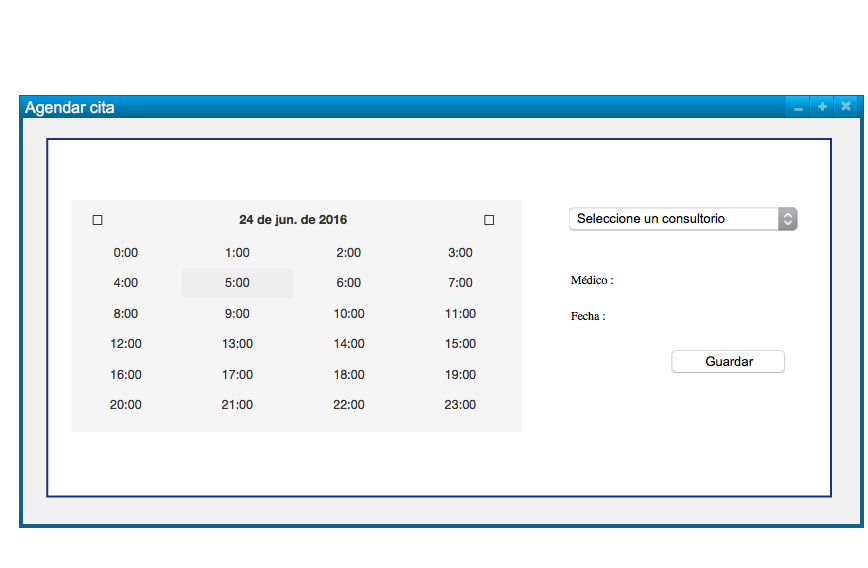
\includegraphics[width=0.8\textwidth]{images/UI2B}
    \caption{Pantalla UI2B Agendar cita}
\end{figure}

\begin{figure}[htbp!]
    \centering
        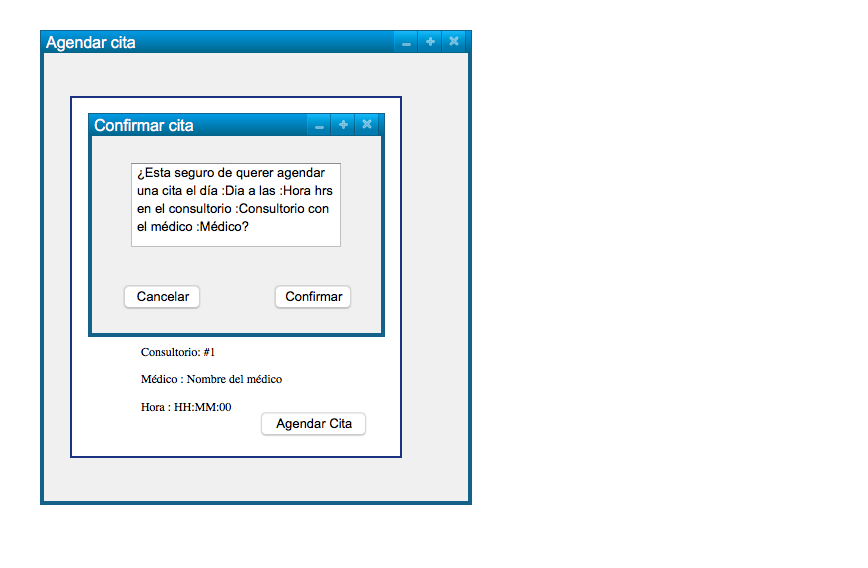
\includegraphics[width=0.8\textwidth]{images/UI2C}
    \caption{Pantalla UI2C Confirmar cita}
\end{figure}
\subsubsection{Entradas}
    \begin{itemize}
        \item Email del paciente: cadena de texto compuesta de 4 partes:  
            \begin{itemize}
                \item cadena de texto.
                \item carácter ‘@’
                \item cadena que identifica al servidor que brinda el servicio de correo electrónico
                \item carácter ‘.’ y dominio
            \end{itemize}
        \item Fecha de cita: cadena de caracteres con el formato ``DD/MM/AAAA'', donde DD, MM y AAAA son número enteros que representan el día, mes y año de la fecha, respectivamente.
        \item Hora de cita: cadena de caracteres con el formato ``HH:MM'' donde HH y MM son números enteros que representan la hora y los minutos de la cita, respectivamente.
        \item Consultorio: Número entero positivo entre 0 y 12, representa el número de consultorio.
    \end{itemize}
\subsubsection{Mensajes}
    \begin{Citemize}
        \item {\bf MSG2a} “Ya se ha agendado una cita con los mismos datos seleccionados”.
    \end{Citemize}

\subsubsection{Comandos}
	\begin{itemize}
	    \item \IUbutton{Día del calendario}: muestra \IUref{UI2B}{Agendar Cita}. 
	    \item \IUbutton{Agendar cita}: muestra \IUref{UI2C}{Confirmar Cita}. 
	    \item \IUbutton{Cancelar}: regresa a \IUref{UI2B}{Agendar Cita}. 
	    \item \IUbutton{Confirmar}: Verifica que no haya agendada una cita con los mismos datos seleccionados. Si la verificación es correcta muestra \IUref{UI3}{Consultar citas}.  
	\end{itemize}

\subsection{IU11 Crear tratamiento}

\subsubsection{Objetivo}
Permitir al médico dar un tratamiento a un paciente.

\subsubsection{Diseño}
Esta pantalla aparece al presionar el botón ``Crear tratamiento'' en \IUref{UI27}{Dar consulta}.   

\begin{figure}[htbp!]
    \centering
        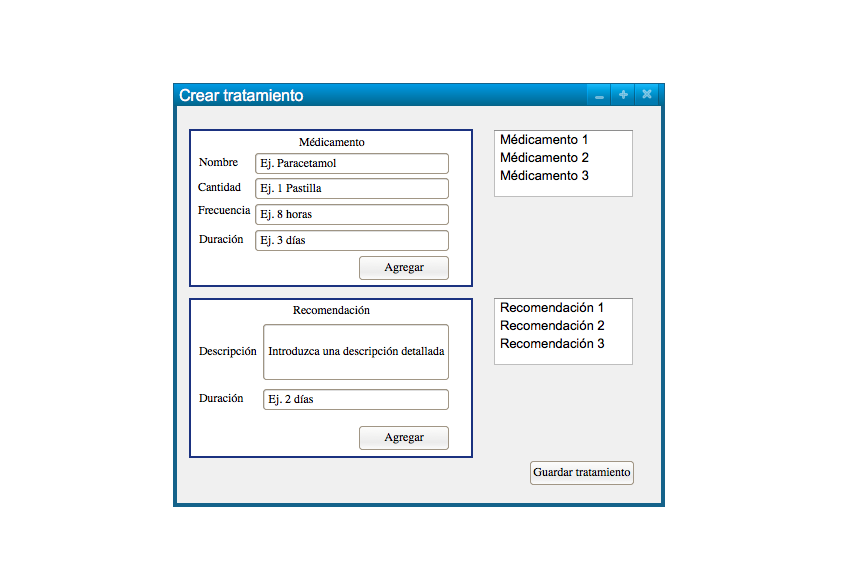
\includegraphics[width=0.8\textwidth]{images/UI11}
    \caption{Pantalla UI11 Crear tratamiento}
\end{figure}

\subsubsection{Entradas}
    \begin{itemize}
      \item Id de consulta: número entero positivo que representa la consulta a la que esta asociada el tratamiento.
      \item Lista de médicamentos: Arreglo de estructuras de datos que contienen lo siguiente:
        \begin{itemize}
          \item Nombre del médicamento: Cadena de caracteres que hacen referencia al nombre comercial del médicamento.
          \item Frecuencia: cadena de carácteres compuesta por un número entero positivo; número de veces en las que se debe tomar el medicamento.
          \item Duración: cadena de carácteres que puede estar compuesta por un número entero positivo que represente el tiempo que debe transcurrir desde que el paciente debe empezar a tomar el médicamento hasta que lo deje de consumir y una unidad de medida. 
          \item Cantidad: cadena de carácteres que puede estar compuesta por número entero positivo y la unidad minima de la presentación del medicamento (Ej. pastilla, mililitros, etc); representa la dosis del médicamento que debe consumir el paciente.

        \end{itemize}   
      \item Lista de recomendaciones: Arreglo de estructuras de datos que contienen lo siguiente:
        \begin{itemize}
          \item Descripción: cadena larga de texto en la que se menciona una recomendación o sugerencia que el paciente debe seguir parar mejorar su estado de salúd.
          \item Duración: cadena de carácteres que puede estar compuesta por un número entero positivo que represente el tiempo que debe transcurrir desde que el paciente debe empezar a seguir la recomendación hasta que sea necesario y una unidad de medida. 
        \end{itemize}   
    \end{itemize}

\subsubsection{Mensajes}
    \begin{Citemize}
        \item {\bf MSG11a} ``Registro del tratamiento exitoso".
      	\item {\bf MSG11b} ``Complete todos los campos del medicamento".
      	\item {\bf MSG11c} ``Complete todos los campos de la recomendación".
      	\item {\bf MSG11d} ``Formato de campos inválido''
    \end{Citemize}

\subsubsection{Comandos}
	\begin{itemize}
	    \item \IUbutton{Agregar} medicamento: añade a la lista de medicamentos los datos del medicamento actual. 
	    \item \IUbutton{Agregar} recomendación: añade a la lista de recomendaciones los datos de la recomendación actual.
	    \item \IUbutton{Guardar tratamiento}: guarda el tratamiento y regresa a \IUref{UI27}{Dar consulta}. 
	\end{itemize}

